\documentclass[fleqn]{article}

\usepackage[latin1]{inputenc}
\usepackage{amsfonts}
\usepackage{amsmath}
\usepackage{dsfont}
\usepackage{german}
\usepackage{graphicx}
\usepackage{tikz}
\usetikzlibrary{arrows,shapes,trees,decorations.pathmorphing,patterns}

\topmargin-25mm
\textheight250mm
\textwidth170mm
\oddsidemargin-10mm
\evensidemargin0mm
\def\ds{\displaystyle}
\def\ty{\scriptscriptstyle}
\mathindent2cc
\parindent0em
\parskip0ex
%\pagestyle{headings}

\begin{document}

{\Large\bf Virialsatz in der Schule}

\bigskip

Idee: Experimentieren mit einer Computersimulation zum empirischen Entdecken/Nachweisen des Virialsatzes anhand einer sich in der horizontalen Ebene reibungsfrei bewegenden Masse, die durch eine Feder mit einem Punkt der Ebene verbunden ist (siehe Skizze).

\pgfdeclarepatternformonly{zigzag}
{\pgfpointorigin}{\pgfpoint{1cm}{1cm}}
{\pgfpoint{0.3cm}{0.3cm}}
{
\tikz\draw[decoration = {zigzag,segment length = 2mm, amplitude = 2mm}, decorate] (0,0) -- ++(3,0);
}

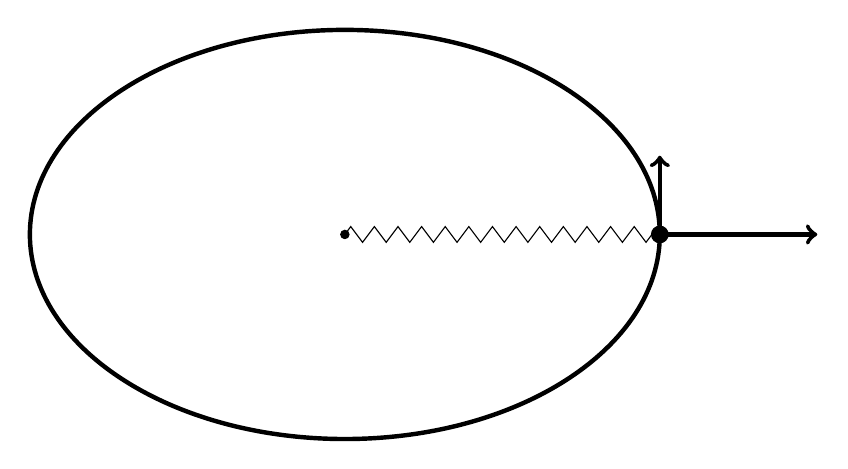
\begin{tikzpicture}
\draw[ultra thick] (0,0) ellipse (4 and 2.598);

\tikzstyle{vertex}=[draw,circle,fill=black,minimum size=6pt,inner sep=0pt]
\draw (4,0) node[vertex] (v) {};

\tikzstyle{vertex}=[draw,circle,fill=black,minimum size=3pt,inner sep=0pt]
\draw (0,0) node[vertex] (v) {};

\draw [->,ultra thick] (4,0) -- (6,0);
\draw [->,ultra thick] (4,0) -- (4,1);
\draw[decoration = {zigzag,segment length = 3mm, amplitude = 1mm},decorate] (0,0)--(4,0);
\end{tikzpicture}

Experimentell k�nnen vor jedem Ablauf der graphisch simulierten Bewegung die Anfangsimpulse $p_{r} = m \dot{r}$ in radialer bzw. $p_{\varphi} = m r^{2} \dot{\varphi}$ in tangentialer Richtung (bzw. Gesamtimpuls) sowie die Federkonstante $D$ als Parameter ver�ndert werden. W�hrend des Programmablaufs werden nummerisch $<T>$ und $<V>$ bestimmt.

Nachdem $<T>$ und $<V>$ bei der Variation der Anfangsbedingungen in der Regel verschiedene Werte liefern, gelingt der Nachweis des Virialsatzes durch Quotientenbildung und Feststellung

\[
\frac{<T>}{<V>} = const.
\].


\end{document}
